\documentclass[utf8]{report}
\usepackage[utf8]{inputenc}
\usepackage[english,russian]{babel}
\usepackage{times, graphicx}
 
\begin{document}

\title{Реализация}
\author{Blokhin Yuri\\
        \texttt{ultrablox@gmail.com}}
\date{\today}
\maketitle
 
\tableofcontents

\begin{abstract}
Данный документ дает детальное реализации компонентов проекта.
\end{abstract}

\chapter{Модуль шасси}

\section{Архитектура}


\begin{figure}
    \centering
    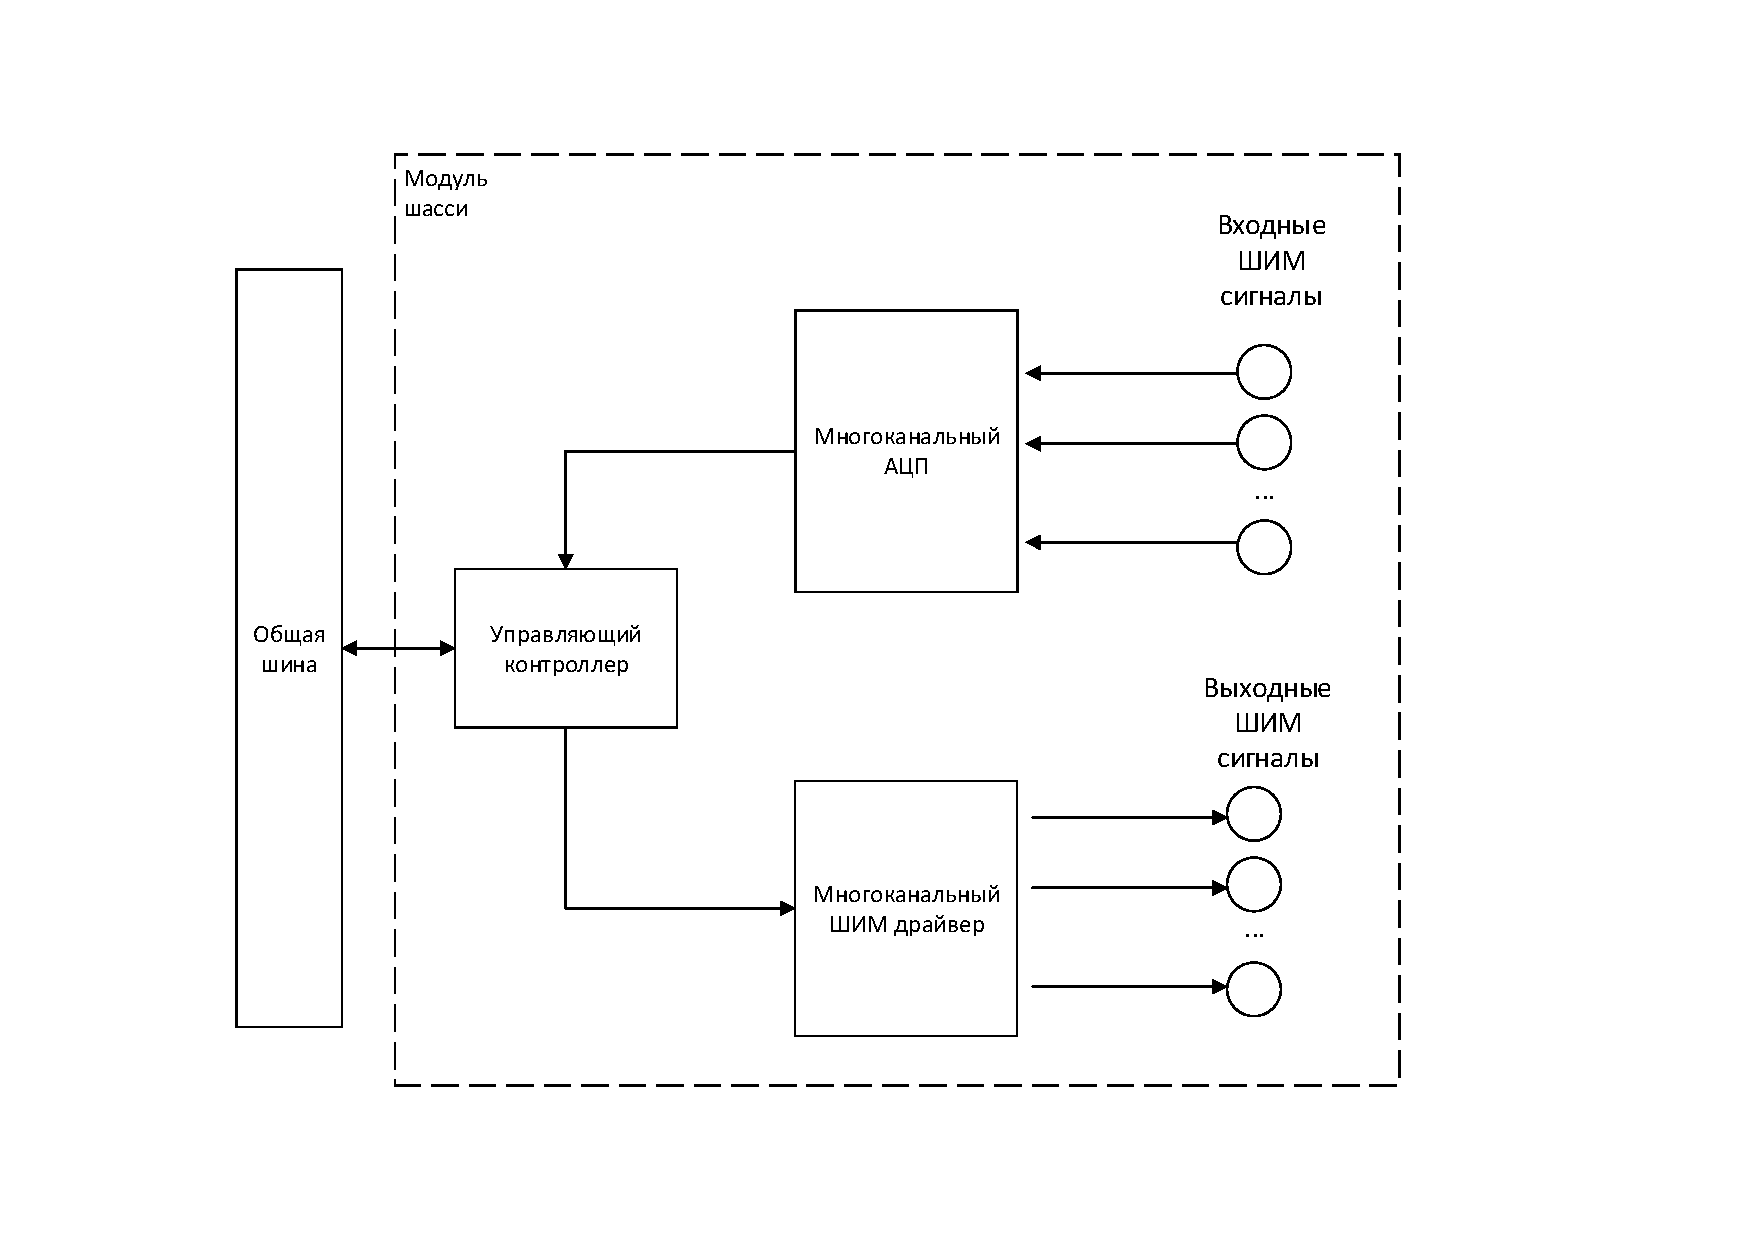
\includegraphics[width=1.2\textwidth]{drawings/chassis_architecture.pdf}
    \caption{Архитектура модуля шасси}
    \label{fig:hashset}
\end{figure}

\section{Выбор электронных комонентов}

\section{Схемы}

\begin{thebibliography}{9}

\end{thebibliography}
 
\end{document}
